\documentclass[12pt]{article}
\usepackage{statproj}

\definecolor{myblue}{HTML}{4c72b0}
\definecolor{myorange}{HTML}{dd8452}
\definecolor{mygreen}{HTML}{55a868}

\title{A Log-Linear Regression Analysis of Allometric Scaling and Species Effects on Penguin Body Mass}
\author{Avigyan Chakraborty}
\date{April, 2026}

\begin{document}

  \maketitlepage{\thetitle}{\theauthor}{\thedate}{%
    This project studies the relationship between penguin body mass
    and selected morphological traits using the Palmer Penguins
    dataset. The response variable is body mass, while flipper
    length, culmen length, culmen depth, and species are used as
    predictors. Since biological measurements often follow
    multiplicative scaling relationships, both the response and
    the continuous predictors are log-transformed, yielding a
    multiple log-linear regression model.

    Species is incorporated through dummy variables, with Adelie
    taken as the baseline category. The fitted model is estimated
    using Ordinary Least Squares and explains a substantial
    proportion of the variation in log body mass, with
    $R^2 = 0.8353$ and adjusted $R^2 = 0.8328$. All predictors
    except the intercept are statistically significant at the
    5\% level.

    Confidence intervals, prediction intervals, and hypothesis
    tests are constructed and interpreted. Residual diagnostics,
    including plots, a normal Q-Q plot, and a chi-square
    goodness-of-fit test, suggest that the assumptions of the
    log-linear model are reasonably satisfied. The analysis shows
    that penguin body mass is strongly associated with
    morphological traits and species membership.%
    }

  \makecontents

  \section{Introduction}

  Understanding how body mass relates to physical
  characteristics is a central problem in biological data
  analysis. Structural measurements such as flipper length and
  bill dimensions are often closely linked to overall size.
  Studying these relationships helps in both prediction and in
  understanding biological variation across species.

  In this project, we analyze the Palmer Penguins dataset,
  which contains measurements of penguins from the Palmer
  Archipelago, Antarctica. The objective is to model body mass
  using flipper length, culmen length, culmen depth, and
  species. Since both continuous and categorical predictors are
  present, multiple linear regression provides a natural
  framework.

  Biological traits frequently exhibit multiplicative scaling,
  rather than purely additive relationships. To account for
  this, a log transformation is applied to the response and the
  continuous predictors. This leads to a log-linear model that
  is both statistically convenient and biologically motivated
  through allometry.

  The analysis begins with a description of the data and
  variables. A regression model is then specified using
  log-transformed predictors and dummy variables for species.
  The model is estimated using Ordinary Least Squares, followed
  by interpretation of coefficients, construction of
  confidence and prediction intervals, and hypothesis testing.
  Finally, residual diagnostics are used to assess the
  validity of the model assumptions.

  \section{Data Description}

  The dataset used in this study is the
  Palmer Penguins dataset.
  It contains morphological measurements of
  penguins observed in the
  Palmer Archipelago, Antarctica.
  It includes data for three species:
  Adelie, Chinstrap, and Gentoo.

  \begin{itemize}
      \ii \textbf{Body Mass (grams)}:
      The weight of the penguin,
      which serves as the response (dependent) variable.
      \ii \textbf{Flipper Length (mm)}:
      The length of the penguin’s flipper, used as a predictor.
      \ii \textbf{Culmen Length (mm)}:
      The length of the penguin’s bill (beak),
      measured along the top ridge,
      used as a predictor.
      \ii \textbf{Culmen Depth (mm)}:
      The depth (height) of the penguin’s bill,
      used as a predictor.
      \ii \textbf{Species}:
      A categorical variable indicating the
      species of the penguin
      (Adelie, Chinstrap, or Gentoo),
      also used as a predictor.
  \end{itemize}

  The dataset initially contained a small number of
  missing values in some of the numerical variables.
  These observations were removed prior to analysis to
  ensure consistency and reliability of the
  regression models.

  The variables selected for this study are
  biologically relevant, as body mass is expected to be
  influenced by structural features such as flipper size
  and bill dimensions,
  along with species-specific characteristics.

  \subsection{Summary Statistics}

  \begin{table}[H]
    \centering
    \begin{tabular}{|| c | c | c | c | c ||}
      \hline
      \textbf{Variable} & \textbf{Mean}
      & \textbf{Minimum}
      & \textbf{Maximum} & \textbf{Std. Dev.} \\[0.5ex]
      \hline\hline
      \textbf{Body Mass (g)} & 4201.754 & 2700 & 6300 & 801.9545 \\
      \textbf{Flipper Length (mm)} & 200.9152 & 172 & 231 & 14.06171 \\
      \textbf{Culmen Length (mm)} & 43.92193 & 32.1 & 59.6 & 5.459584 \\
      \textbf{Culmen Depth (mm)} & 17.15117 & 13.1 & 21.5 & 1.974793 \\
      \hline
    \end{tabular}
    \caption{Overall Summary Statistics}
  \end{table}

  \begin{table}[H]
    \centering
    \begin{tabular}{|| c | c | c | c | c | c ||}
      \hline
      \textbf{Species}
      & \textbf{Variable} & \textbf{Mean}
      & \textbf{Minimum}
      & \textbf{Maximum} & \textbf{Std. Dev.} \\[0.5ex]
      \hline\hline
      \multirow{4}{*}{\begin{tabular}{c}
        \textbf{Adelie} \\
        \textbf{(151)}
      \end{tabular}}
      & \textbf{Body Mass (g)} & 3700.662 & 2850 & 4775 & 458.5661 \\
      & \textbf{Flipper Length (mm)} & 189.9536 & 172 & 210 & 6.539457 \\
      & \textbf{Culmen Length (mm)} & 38.79139 & 32.1 & 46 & 2.663405 \\
      & \textbf{Culmen Depth (mm)} & 18.34636 & 15.5 & 21.5 & 1.21665 \\
      \hline
      \multirow{4}{*}{\begin{tabular}{c}
        \textbf{Gentoo} \\
        \textbf{(123)}
      \end{tabular}}
      & \textbf{Body Mass (g)} & 5076.016 & 3950 & 6300 & 504.1162 \\
      & \textbf{Flipper Length (mm)} & 217.187 & 203 & 231 & 6.484976 \\
      & \textbf{Culmen Length (mm)} & 47.50488 & 40.9 & 59.6 & 3.081857 \\
      & \textbf{Culmen Depth (mm)} & 14.98211 & 13.1 & 17.3 & 0.9812198 \\
      \hline
      \multirow{4}{*}{\begin{tabular}{c}
        \textbf{Chinstrap} \\
        \textbf{(68)}
      \end{tabular}}
      & \textbf{Body Mass (g)} & 3733.088 & 2700 & 4800 & 384.3351\\
      & \textbf{Flipper Length (mm)} & 195.8235 & 178 & 212 & 7.131894 \\
      & \textbf{Culmen Length (mm)} & 48.83382 & 40.9 & 58 & 3.339256 \\
      & \textbf{Culmen Depth (mm)} & 18.42059 & 16.4 & 20.8 & 1.135395 \\
      \hline
    \end{tabular}
    \caption{Summary Statistics of Species}
  \end{table}

  \subsection{Data Source}

  The dataset used in this study is the Palmer Penguins\cite{palmerpenguins}
  dataset, originally provided by Dr. Kristen Gorman. It is
  available via the GitHub repository:
  \href{https://github.com/allisonhorst/palmerpenguins/tree/main}
  {palmerpenguins (GitHub)}, and is also hosted on Kaggle:
  \href{https://www.kaggle.com/datasets/parulpandey/palmer-archipelago-antarctica-penguin-data}
  {Palmer Archipelago Penguin Data (Kaggle)}.

  \section{Model Specification}

  \subsection{Theoretical Motivation}

  Biological traits (such as beak dimensions, flipper length,
  and body mass) scale proportionally relative to one another,
  a phenomenon known as allometry.
  This proportional, multiplicative growth is
  mathematically represented by a
  non-linear power law equation: $Y = \alpha X^{\beta}$.

  Ordinary Least Squares (OLS) regression can only
  fit strictly linear relationships.
  By applying a natural logarithm to both sides of the
  allometric power law, we algebraically transform the
  biological curve into a perfectly straight line:
  \[
    \log(Y) = \log(\alpha) + \beta \log(X)
    .\]
  This mathematical linearization allows the standard OLS model
  to accurately capture and estimate the proportional scaling rate
  $(\beta)$ as a simple additive slope.

  \subsection{Model Structure and Variable Encoding}

  First, we briefly introduce categorical variables before putting them
  to use. Unlike continuous variables
  (such as Flipper Length or Body Mass) which represent measurable,
  numerical quantities, categorical variables
  represent qualitative groups or labels (such as Penguin Species).
  Ordinary Least Squares (OLS) regression relies on
  strictly numerical equations.
  Therefore, categorical variables must be mathematically transformed
  before they can be included in a linear model.

  To incorporate qualitative data, statistical models
  utilize Dummy Variables (also known as One-Hot Encoding).
  This process translates categorical labels into a series of
  binary variables, assigning a $1$ if the condition is met
  and a $0$ if it is not.

  In context of our current dataset, we are going to
  use the following categorical variables:
  \begin{itemize}
      \ii \texttt{Is\_Gen}: $1$ if Gentoo, $0$ otherwise.
      \ii \texttt{Is\_Chin}: $1$ if Chinstrap, $0$ otherwise.
  \end{itemize}
  The baseline, Adelie, is mathematically implied when both
  \texttt{Is\_Gen} and \texttt{Is\_Chin} are equal to $0$.
  We do not account for this separately in the model as
  its effect is absorbed directly
  into the model's intercept, $\beta_0$.

  Our objective is to predict the response variable,
  \texttt{Body\_M}, using the predictors \texttt{Flip\_L},
  \texttt{Culm\_L}, \texttt{Culm\_D}, \texttt{Is\_Gen}, and
  \texttt{Is\_Chin}. We have $n=342$ row entries in our dataset and
  $p=5$ many parameters.
  Clearly $n > p+1$. Furthermore,
  if we let $X$ be the $n \times (p+1)$ order matrix
  where the first column has all entries $1$ and the other columns
  have row-wise entries of the values of the predictors
  stated above, in order, then $X$ has full column rank.
  Thus, the model is estimable and does not suffer from
  perfect multicollinearity.
  The remaining regression assumptions are assessed
  through residual diagnostics.

  We shall now verify the credibility of the normality assumption
  of the errors. First, we fit a model using the raw data from our
  dataset and then compare it with the model fitted by using
  the log-transformed data.

  We know that $\hat{\beta}$ is given by $(X\trans X)^{-1} X\trans Y$.
  Plugging in the values for the raw data, we get that
  \[
    \hat{\beta}_{\text{raw}}
    = (-4327.327, 20.241, 41.468, 140.328, 934.887, -513.247)\trans
  \]
  for which the corresponding fitted model is
  \begin{align*}
    \widehat{\texttt{Body\_M}} = -4327.327
    + 20.241\cdot\texttt{Flip\_L}
    &+ 41.468\cdot\texttt{Culm\_L}
    + 140.328\cdot\texttt{Culm\_D} \\
    &+ 934.887\cdot\texttt{Is\_Gen}
    -513.247\cdot\texttt{Is\_Chin}
  .\end{align*}

  So, the residuals, $\hat{\eps}_i$ are given by
  $\texttt{Body\_M}_i - \widehat{\texttt{Body\_M}_i}$.
  Two residual plots for the raw model are shown below:
  a plot of residuals against observation index,
  and a histogram of the residuals.
  \begin{figure}[H]
    \centering
    \begin{minipage}{0.45\textwidth}
      \centering
      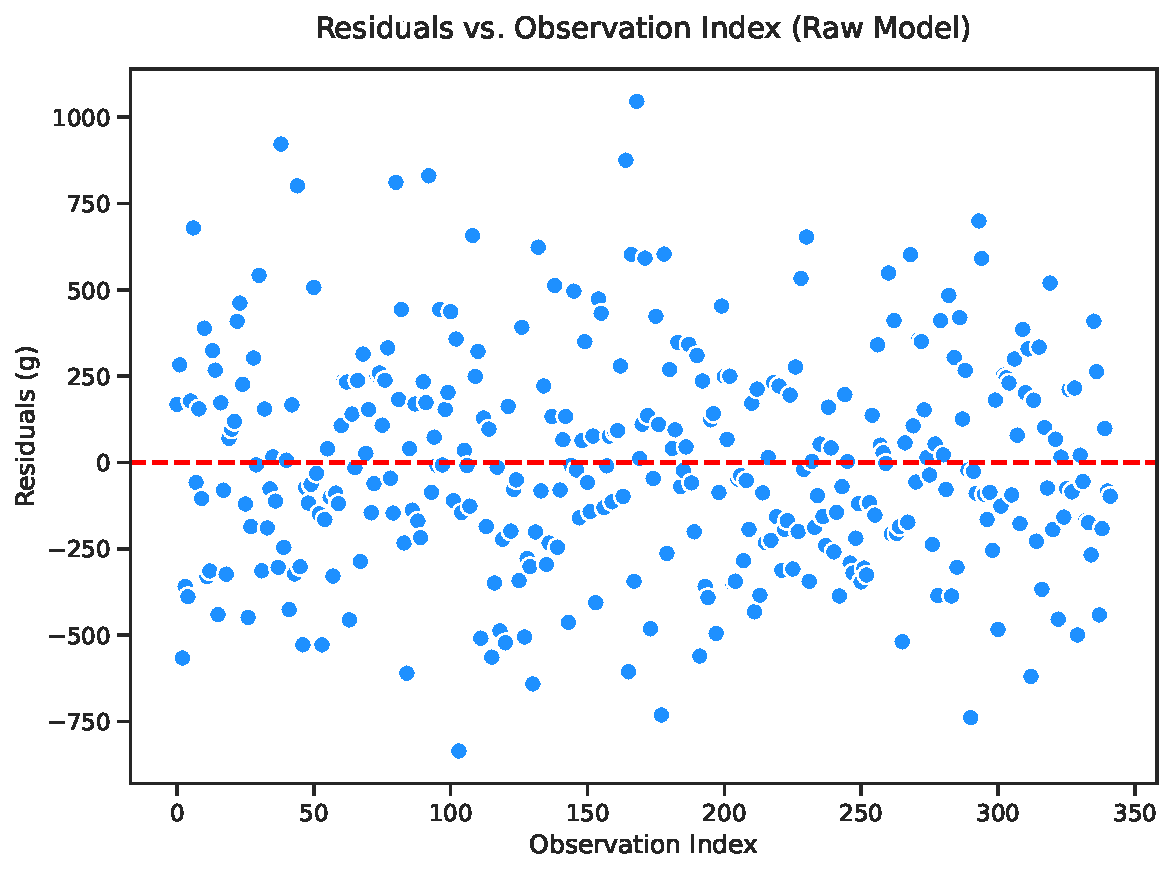
\includegraphics[width=0.9\textwidth,keepaspectratio]{./codes/plots/model-formulation/raw-res-plot.pdf}
      \caption{Plot of Residuals vs. Observation Index for the Raw Model}
    \end{minipage}\hfill
    \begin{minipage}{0.45\textwidth}
      \centering
      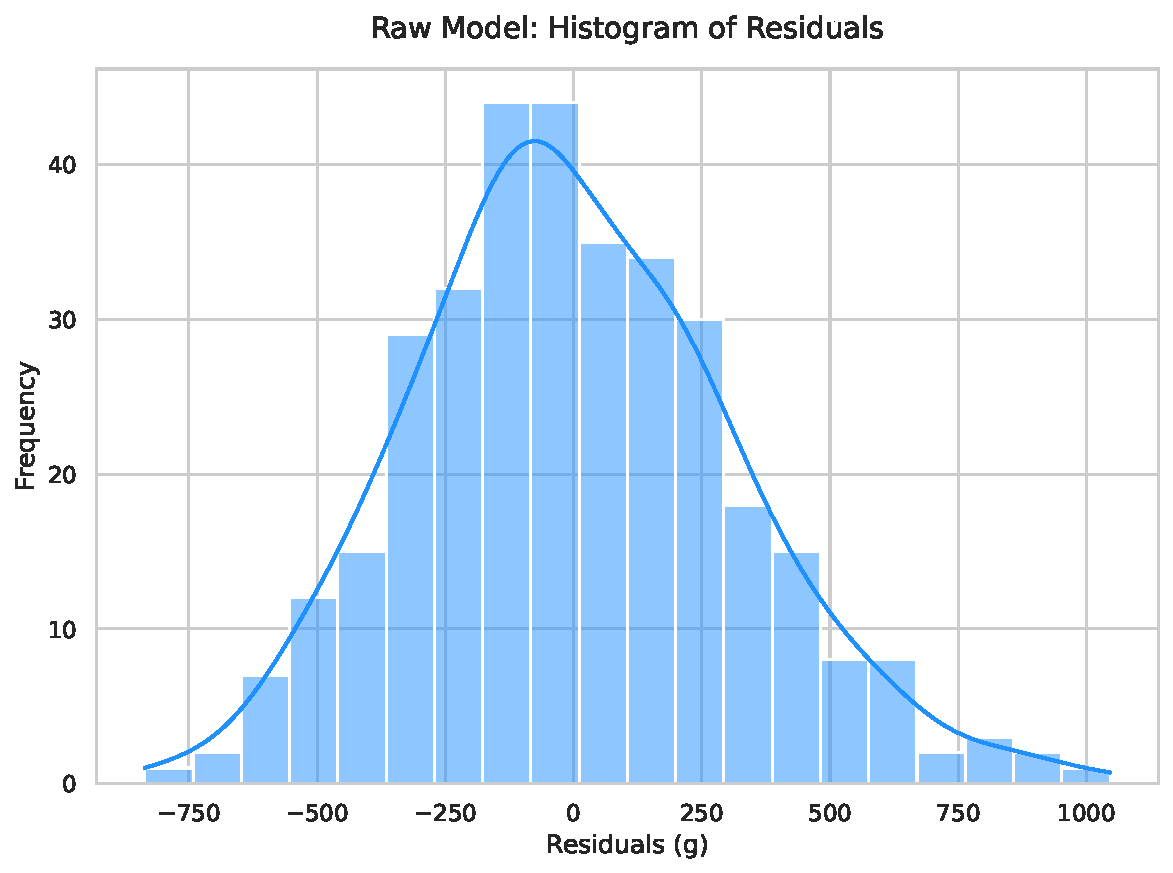
\includegraphics[width=0.9\textwidth,keepaspectratio]{./codes/plots/model-formulation/raw-res-hist.pdf}
      \caption{Histogram of Residuals for the Raw Model}
      \label{figure:raw_res_hist}
    \end{minipage}
  \end{figure}

  As it can be noted, in the histogram plot of the residuals
  (\cref{figure:raw_res_hist}),
  the distribution is skewed towards the right. Thus, this might
  pose problems for the normality assumption.

  Now, let us work with the log-transformed model. Proceeding similarly
  as before, we get
  \[
    \hat{\beta}_{\text{log}}
    = (0.07590, 0.90358, 0.43644, 0.61806, 0.23408, -0.11952)\trans
  \]
  for which the corresponding fitted model is
  \begin{align*}
    \widehat{\log(\texttt{Body\_M})} = 0.07590
    &+ 0.90358\cdot\log(\texttt{Flip\_L})
    + 0.43644\cdot\log(\texttt{Culm\_L}) \\
    &+ 0.61806\cdot\log(\texttt{Culm\_D})
    + 0.23408\cdot\texttt{Is\_Gen}
    -0.11952\cdot\texttt{Is\_Chin}
  .\end{align*}
  In this case, the residuals, $\hat{\eps}_{i}$ are given by
  $\log(\texttt{Body\_M}_i) - \widehat{\log(\texttt{Body\_M}_i)}$.
  Two residual plots for the log-transformed model are shown below:
  a plot of residuals against observation index,
  and a histogram of the residuals.
  \begin{figure}[H]
    \centering
    \begin{minipage}{0.45\textwidth}
      \centering
      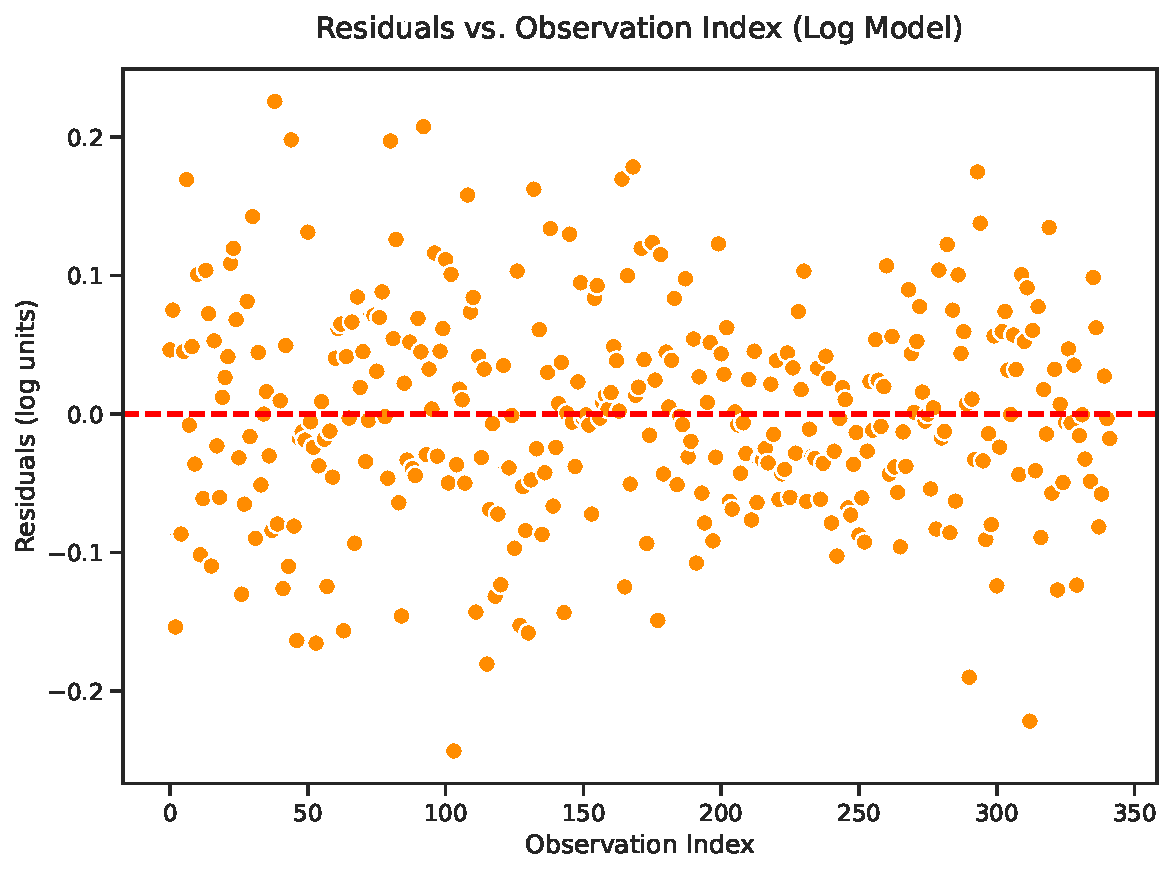
\includegraphics[width=0.9\textwidth,keepaspectratio]{./codes/plots/model-formulation/log-res-plot.pdf}
      \caption{Plot of Residuals vs. Observation Index for Log Model}
    \end{minipage}\hfill
    \begin{minipage}{0.45\textwidth}
      \centering
      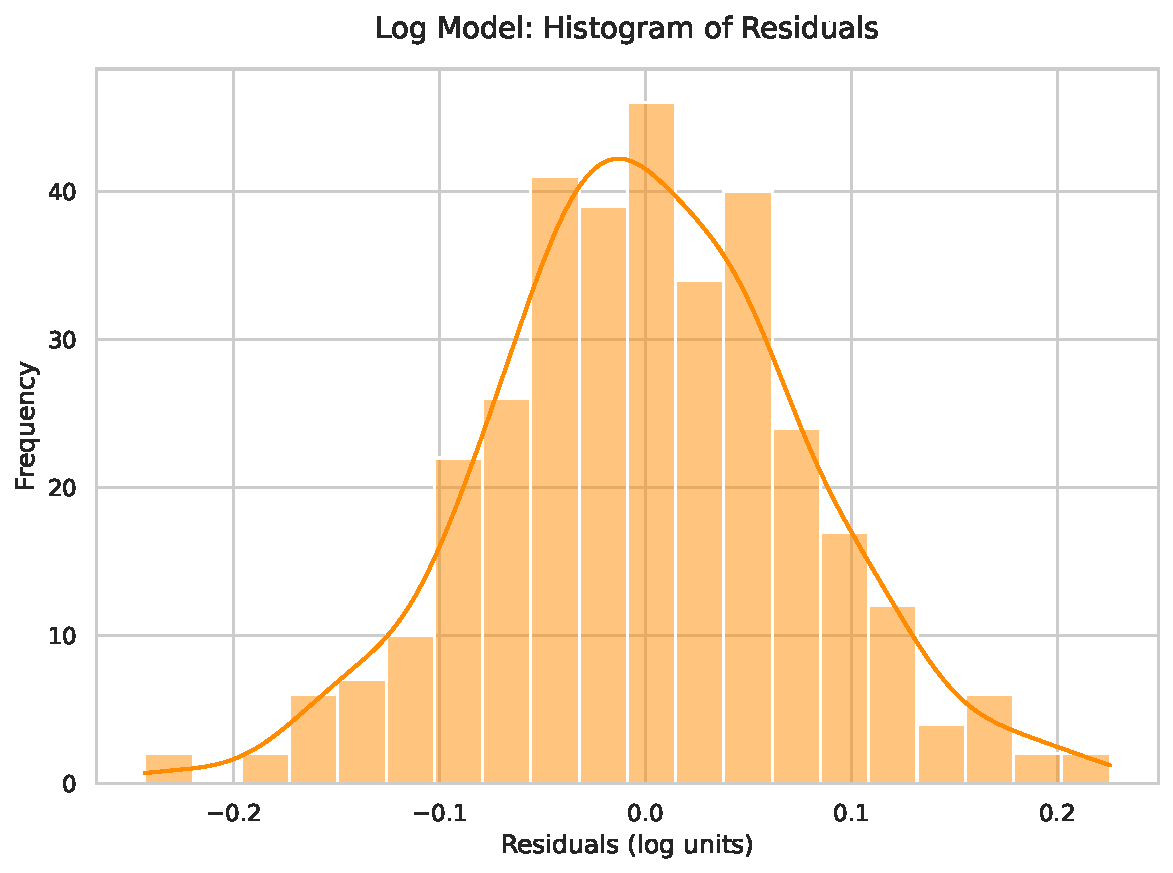
\includegraphics[width=0.9\textwidth,keepaspectratio]{./codes/plots/model-formulation/log-res-hist.pdf}
      \caption{Histogram of Residuals for the Log Model}
      \label{figure:log_res_hist}
    \end{minipage}
  \end{figure}

  In the histogram of the log-transformed model
  (\cref{figure:log_res_hist}),
  the curve looks almost perfectly symmetric
  and the left and right tails mirror each other
  around the center zero mark.

  This suggests us that using the log-transformed data would be
  better suited to our needs. We shall further verify
  the goodness of this fit test in \cref{subsection:goodness_of_fit}.

  \section{Model Estimation and Results}

  \subsection{Estimated Model}
  The Multiple Linear Regression (MLR) model was fitted
  to the data using Ordinary Least Squares (OLS) estimation.
  As established in the previous section,
  the fitted regression equation utilizes log-transformed
  continuous variables to linearize the underlying
  allometric scaling relationships, and is represented as:
  \begin{align*}
    \widehat{\log(\texttt{Body\_M})} = 0.07590
    &+ 0.90358\cdot\log(\texttt{Flip\_L})
    + 0.43644\cdot\log(\texttt{Culm\_L}) \\
    &+ 0.61806\cdot\log(\texttt{Culm\_D})
    + 0.23408\cdot\texttt{Is\_Gen}
    -0.11952\cdot\texttt{Is\_Chin}
  .\end{align*}

  The following scatterplot matrix shows the pairwise relationship
  between our different variables used for this study:
  \begin{figure}[H]
    \centering
    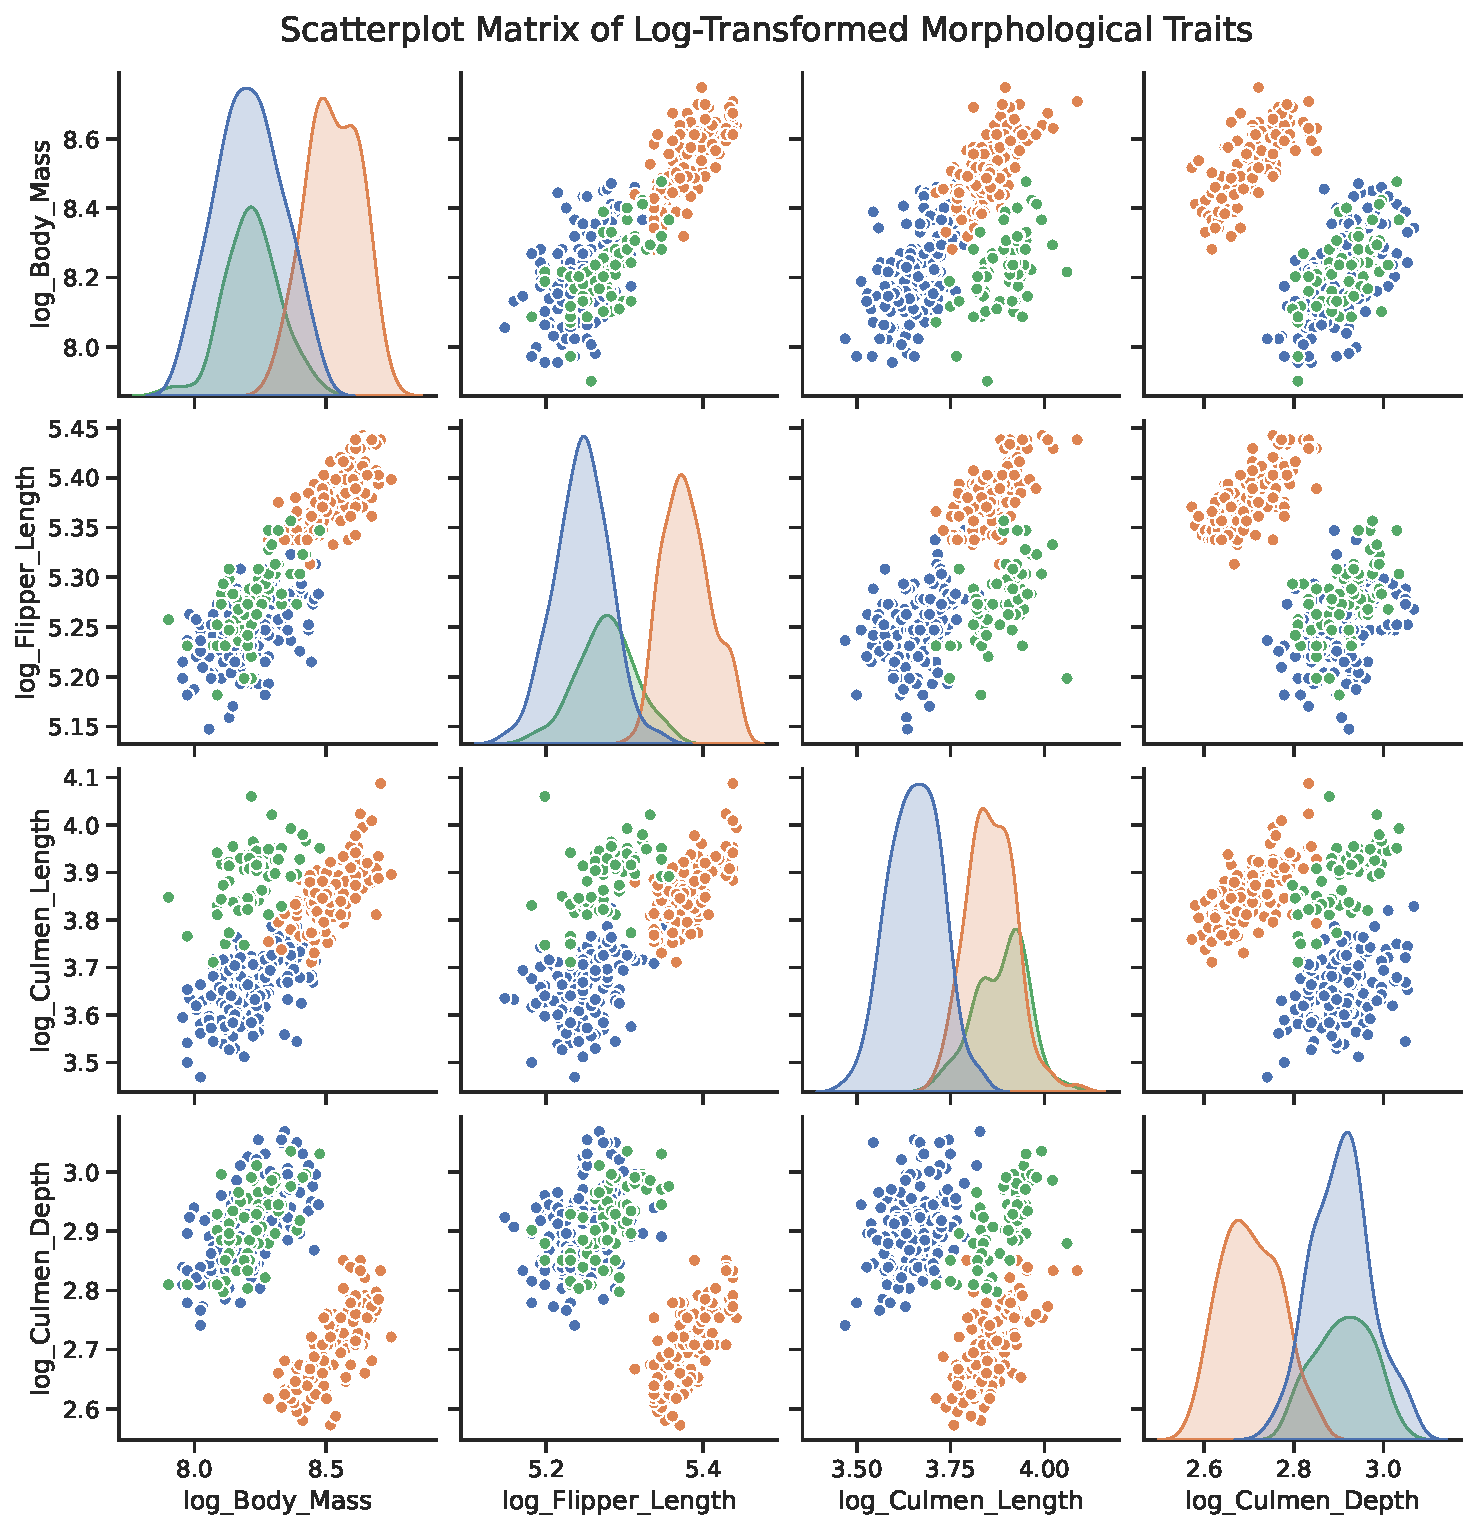
\includegraphics[width=\textwidth,keepaspectratio]{./codes/plots/model-analysis/splom.pdf}
    \caption{Scatterplot matrix of log-transformed morphological traits.
    Data points and density distributions are colored by species:
    Adelie (\textcolor{myblue}{blue}),
    Gentoo (\textcolor{myorange}{orange}),
    and Chinstrap (\textcolor{mygreen}{green}).}
  \end{figure}

  \subsection{Regression Results}
  The results of the regression analysis,
  including the estimated coefficients, standard errors,
  and corresponding p-values, are summarized in \cref{table:reg_output}.
  The model is highly robust, explaining approximately $83.5\%$
  of the variance in the log-transformed body mass of the $342$
  penguins sampled ($R^2 = 0.8353$).

  \begin{table}[H]
    \centering
    \begin{tabular}{|| c | c | c | c ||}
      \hline
      \textbf{Predictor Variable}
      & \textbf{Coefficient} ($\hat{\beta}$)
      & \textbf{Std. Error}
      & \textbf{p-value} \\[0.5ex]
      \hline\hline
      \texttt{Intercept} ($\hat{\beta}_0$) & 0.07590 & 0.677 & 0.911 \\
      $\log(\texttt{Flip\_L})$ ($\hat{\beta}_1$) & 0.90358 & 0.149 & $< 0.001$ \\
      $\log(\texttt{Culm\_L})$ ($\hat{\beta}_2$) & 0.43644 & 0.076 & $< 0.001$ \\
      $\log(\texttt{Culm\_D})$ ($\hat{\beta}_3$) & 0.61806 & 0.080 & $< 0.001$ \\
      \texttt{Is\_Gen} ($\hat{\beta}_4$) & 0.23408 & 0.035 & $< 0.001$ \\
      \texttt{Is\_Chin} ($\hat{\beta}_5$) & -0.11952 & 0.020 & $< 0.001$ \\
      \hline
    \end{tabular}
    \caption{OLS Regression Results for Penguin Body Mass}
    \label{table:reg_output}
  \end{table}

  The following correlation matrix shows the correlation between
  the variables used in this study:
  \begin{figure}[H]
    \centering
    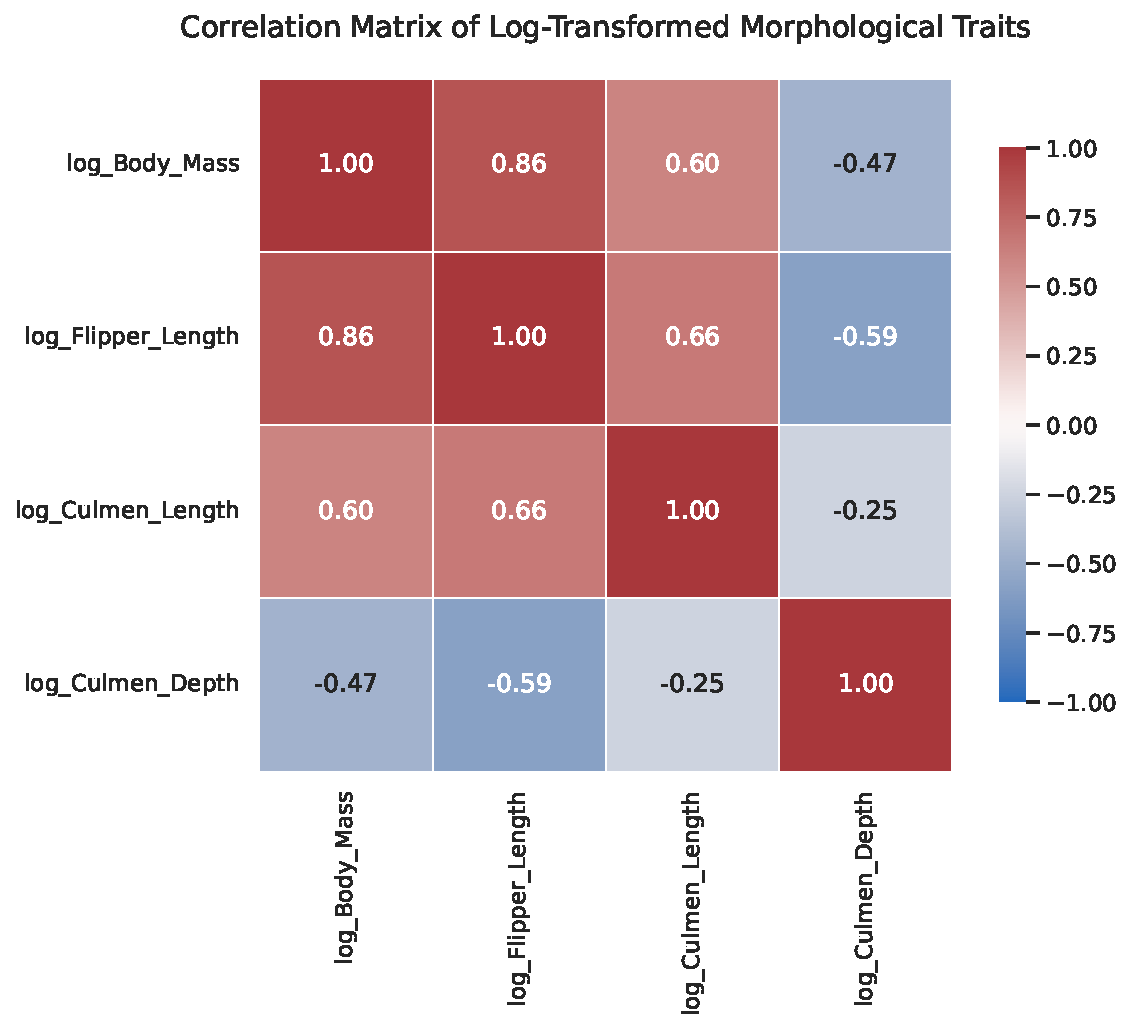
\includegraphics[width=0.8\textwidth,keepaspectratio]{./codes/plots/model-analysis/corr-matrix.pdf}
    \caption{Correlation Matrix of Log-Transformed Morphological Traits}
  \end{figure}

  The correlation matrix of the log-transformed variables reveals
  clear linear relationships among the morphological traits.
  In particular, $\log(\texttt{Body\_M})$ shows a strong positive
  correlation with $\log(\texttt{Flipper\_L})$,
  indicating that larger penguins tend to have longer flippers.
  There is also a moderate positive association between
  $\log(\texttt{Body\_M})$ and $\log(\texttt{Culmen\_L})$,
  suggesting that heavier penguins generally have longer bills.
  In contrast, $\log(\texttt{Culmen\_D})$ exhibits a strong negative
  relationship with $\log(\texttt{Body\_M})$ and other variables,
  suggesting a different structural relationship across species.


  \subsection{Interpretation of Coefficients}
  The regression results provide highly significant
  insights into the physical and
  species-related differences associated with
  penguin body mass.
  Notably, every predictor variable (excluding the baseline intercept)
  proved to be statistically significant at the $\alpha=0.05$ level:

  \begin{itemize}
      \ii \textbf{Allometric Scaling:} All physical dimensions exhibit
      a positive and highly significant relationship with
      $\log(\texttt{Body\_M})$ ($p < 0.001$).
      \begin{itemize}
          \ii For every $1\%$ increase in Flipper Length (\texttt{Flip\_L}),
          body mass (\texttt{Body\_M}) increases by roughly $0.90\%$.
          \ii For every $1\%$ increase in Culmen Length (\texttt{Culmen\_L}),
          body mass (\texttt{Body\_M}) increases by roughly $0.44\%$.
          \ii For every $1\%$ increase in Culmen Depth (\texttt{Culmen\_D}),
          body mass (\texttt{Body\_M}) increases by roughly $0.62\%$.
      \end{itemize}
      \ii \textbf{Species Genetics:} The inclusion of the
      dummy variables successfully controls for
      underlying genetic differences between the species,
      with Adelie acting as the unstated baseline reference group.
      Both indicator variables are highly significant ($p < 0.001$).
      \begin{itemize}
          \ii The positive coefficient for \texttt{Is\_Gen} ($0.23408$)
          indicates that, assuming identical physical proportions,
          a Gentoo penguin is expected to have approximately
          $26.4\%$
          greater body mass than an Adelie penguin,
          holding other variables constant.
          \ii Conversely, the negative coefficient for
          \texttt{Is\_Chin} ($-0.11952$) dictates that,
          assuming identical physical proportions,
          a Chinstrap penguin is expected to have approximately
          $-11.3\%$
          lower body mass than an Adelie penguin,
          holding other variables constant.
      \end{itemize}
  \end{itemize}

  \section{Statistical Inference}

  \subsection{Confidence Intervals}

  In multiple linear regression,
  estimating the point values for the coefficients
  $(\hat{\beta}_i)$ provides a single best guess for the
  population parameters. However,
  to account for sampling variability and quantify the
  precision of these estimates, we construct $95\%$
  confidence intervals for each predictor, the mean response,
  and future individual observations.

  \subsubsection{Coefficient Intervals}
  The true parameter $(\hat{\beta}_i)$ is estimated to fall
  within the following interval with a $95\%$ level of confidence:
  \[
    \hat{\beta}_i \pm t_{{\alpha}/{2}}(n-p-1)\cdot SE(\hat{\beta}_i)
    .\]
  Plugging in the values, we derive the following interval estimates:
  \begin{table}[H]
    \centering
    \begin{tabular}{|| c | c | c c ||}
      \hline
      \textbf{Predictor Variable}
      & \textbf{Estimate}
      & \textbf{Lower Bound ($2.5\%$)}
      & \textbf{Upper Bound ($97.5\%$)} \\[0.5ex]
      \hline\hline
      \texttt{Intercept} ($\hat{\beta}_0$) & 0.0759 & -1.2559 & 1.4077 \\
      $\log(\texttt{Flipper\_Length})$ ($\hat{\beta}_1$) & 0.9036 & 0.6099 & 1.1972 \\
      $\log(\texttt{Culmen\_Length})$ ($\hat{\beta}_2$) & 0.4364 & 0.2864 & 0.5865 \\
      $\log(\texttt{Culmen\_Depth})$ ($\hat{\beta}_3$) & 0.6181 & 0.4598 & 0.7763 \\
      \texttt{Is\_Gen} ($\hat{\beta}_4$) & 0.2341 & 0.1648 & 0.3034 \\
      \texttt{Is\_Chin} ($\hat{\beta}_5$) & -0.1195 & -0.1592 & -0.0798 \\
      \hline
    \end{tabular}
    \caption{$95\%$ Confidence Intervals for the Regression Parameters}
  \end{table}

  Because both the response variable and the continuous predictors were
  log-transformed, the coefficients are interpreted as
  elasticities, representing the expected percentage change in
  body mass for a $1\%$ increase in the predictor,
  holding all other variables constant.
  \begin{itemize}
      \ii \textbf{Flipper Length:} We are $95\%$ confident that for every $1\%$
      increase in a penguin's flipper length,
      its expected body mass increases by between $0.61\%$ and $1.20\%$.

      \ii \textbf{Culmen Length:} We are $95\%$ confident that a $1\%$
      increase in culmen length corresponds to an expected body mass
      increase of between $0.29\%$ and $0.59\%$.

      \ii \textbf{Culmen Depth:} We are $95\%$ confident that a $1\%$
      increase in culmen depth is associated with a
      $0.46\%$ to $0.78\%$ increase in expected body mass.

      \ii \textbf{Species Effects (\texttt{Is\_Gen}):}
      We are $95\%$ confident that,
      holding all physical measurements constant,
      a Gentoo penguin will weigh between $17.9\%$ and $35.4\%$
      more than the baseline Adelie species.

      \ii \textbf{Species Effects (\texttt{Is\_Chin}):}
      We are $95\%$ confident that,
      holding all physical measurements constant,
      a Chinstrap penguin will weigh between $7.7\%$ and $14.7\%$
      less than the Adelie species.

      \ii \textbf{Intercept:} The $95\%$ confidence interval
      for the intercept ranges from $-1.2559$ to $1.4077$.
      The intercept corresponds to the expected
      log body mass of a baseline Adelie penguin
      when all log-transformed predictors are equal to zero.
      This implies that the original
      measurements are equal to 1 (since $\log(1) = 0$),
      which is not biologically meaningful.
      Thus, the intercept has limited practical
      interpretation in this context.
  \end{itemize}

  \subsubsection{Confidence Intervals for the Mean Response}
  Let $x_0$ be
  a column vector containing a specific set of predictor
  values. To estimate the expected value $\mathbb{E}[\log(\texttt{Body\_M})]$ at
  $x_0$, we utilize the matrix $X$
  to account for the covariance among predictors. The $95\%$
  confidence interval for the mean response is given by:
  \[
    \hat{y}_0 \pm t_{\alpha/2}(n-p-1) \cdot
    \sqrt{\text{MSE} \cdot x_0^T
    (X^T X)^{-1} x_0}
    .\]
  Here, MSE is the Mean Squared Error, estimating the error
  variance $\sigma^2$.

  \paragraph{Application: Expected Mass Across Species}
  To isolate the structural effects of the categorical
  variables, we construct a theoretical standardized penguin
  utilizing the mean of the log-transformed morphological
  measurements. We then predict the expected $\log(\texttt{Body\_M})$
  across all three species profiles, keeping these baseline
  log-dimensions mathematically constant.

  \begin{table}[H]
    \centering
    \begin{tabular}{|| c | c | c c ||}
      \hline
      \textbf{Species}
      & \textbf{Point Estimate}
      & \textbf{Lower Bound}
      & \textbf{Upper Bound} \\
      \hline\hline
      \textbf{Adelie (Baseline)} & 8.2651 & 8.2337 & 8.2964 \\
      \textbf{Chinstrap} & 8.1456 & 8.1178 & 8.1733 \\
      \textbf{Gentoo} & 8.4992 & 8.4581 & 8.5402 \\
      \hline
    \end{tabular}
    \caption{$95\%$ Confidence Intervals for Mean Response}
  \end{table}

  Observing the Chinstrap and Gentoo confidence bounds,
  we see parallel shifts relative to the Adelie baseline.
  Because the input traits are identical, we are $95\%$
  confident that the average log body mass of a Gentoo
  population will always remain strictly higher than an
  identically proportioned Adelie population, whereas a
  Chinstrap population will remain strictly lower.


  \subsubsection{Prediction Intervals}
  While the confidence interval predicts
  $\mathbb{E}[\log(\texttt{Body\_M})]$
  for all penguins with a specific set of traits, the
  prediction interval predicts the exact
  $\log(\texttt{Body\_M})$
  of a
  single, individual new penguin. Because individual
  observations naturally vary around the population mean,
  predicting a single point carries additional irreducible
  uncertainty. The $95\%$ prediction interval
  of $\log(\texttt{Body\_M})$ is mathematically
  wider and is expressed as:
  \[
    \hat{y}_0 \pm t_{\alpha/2}(n-p-1) \cdot
    \sqrt{\text{MSE} \cdot \left(1 + x_0^T
    (X^T X)^{-1} x_0\right)}
    .\]
  The addition of $1$ inside the parenthetical term accounts
  for the variance of the residual error ($\sigma^2$)
  associated with drawing a new, random individual from the
  population.

  \paragraph{Application: Predicting Individual Penguins}
  Using the same theoretical baseline log-dimensions, we now
  calculate the intervals for randomly sampling a single new
  penguin from each respective species.

  \begin{table}[H]
    \centering
    \begin{tabular}{|| c | c | c c ||}
      \hline
      \textbf{Species}
      & \textbf{Point Estimate}
      & \textbf{Lower Bound}
      & \textbf{Upper Bound} \\
      \hline\hline
      \textbf{Adelie (Baseline)} & 8.2651 & 8.1107 & 8.4195 \\
      \textbf{Chinstrap} & 8.1456 & 7.9918 & 8.2993 \\
      \textbf{Gentoo} & 8.4992 & 8.3425 & 8.6558 \\
      \hline
    \end{tabular}
    \caption{$95\%$ Prediction Intervals for New Observations}
  \end{table}

  As mathematically expected, these prediction intervals are
  significantly wider than their corresponding confidence
  intervals. This increased width explicitly accounts for the
  inherent random variation ($\sigma^2$) between individual
  penguins, even when they belong to the exact same species
  and share identical physical measurements.


  \subsection{Hypothesis Testing}
  To formally evaluate the explanatory power and structural
  validity of our multiple log-linear regression model, we
  conduct three distinct tiers of hypothesis testing.

  \subsubsection{Overall Model Significance}
  The global F-test evaluates whether the model as a whole
  explains a statistically significant portion of the variance
  in expected log body mass. To do this, we compare the full
  model against a restricted, intercept-only baseline model.
  \begin{itemize}
      \ii \textbf{Null Hypothesis ($H_0$):} $\beta_1 = \beta_2 =
      \beta_3 = \beta_4 = \beta_5 = 0$. None of the predictors
      have a significant linear relationship with the response.

      \ii \textbf{Alternative Hypothesis ($H_1$):} At least one
      $\beta_i \neq 0$ (for $i \in \{1,2,3,4,5\}$).
  \end{itemize}
  The test statistic
  evaluates the reduction in SSE when
  all predictors are added to the intercept model:
  \[
    F_0 = \frac{{(\text{SSE}_{\text{restricted}} -
    \text{SSE}_{\text{full}})} / {\mathrm{df}_{\text{restricted}} -
    \mathrm{df}_{\text{full}}}}{\text{SSE}_{\text{full}}
    / \mathrm{df}_{\text{full}}}
    .\]
  For the global test, the restricted intercept-only model
  has $\mathrm{df} = n-1$, and the full model containing $5$ predictors
  has $\mathrm{df} = n-6$. Evaluating these degrees of freedom, the
  formula simplifies to:
  \[
    F_0 = \frac{(\text{SSE}_{\text{restricted}} -
    \text{SSE}_{\text{full}}) / 5}{\text{SSE}_{\text{full}}
    / 336}
    .\]

  \paragraph{Calculation and Inference}
  Evaluating the global model yields an F-statistic of
  $F_0 = 340.7279$, which corresponds to a p-value strictly
  less than $0.001$. Because
  this p-value is significantly smaller than our significance
  level ($\alpha = 0.05$), we reject the null hypothesis. We
  conclude with $95\%$ confidence that the regression model
  as a whole explains a statistically significant proportion
  of the variance in expected log body mass.


  \subsubsection{Individual Parameter Significance}
  While the global F-test evaluates the entire model, marginal
  t-tests evaluate the independent contribution of each
  specific predictor, holding all other variables constant.
  \begin{itemize}
      \ii \textbf{Null Hypothesis ($H_0$):} $\beta_i = 0$. The
      $i$-th predictor does not significantly affect expected
      log body mass.

      \ii \textbf{Alternative Hypothesis ($H_1$):} $\beta_i \neq 0$.
  \end{itemize}
  The test statistic is calculated by dividing the parameter
  estimate by its standard error:
  \[
    t_0 = \frac{\hat{\beta}_i}{\text{SE}(\hat{\beta}_i)}
    .\]

  \begin{table}[H]
    \centering
    \begin{tabular}{|| c | c | c | c ||}
      \hline
      \textbf{Predictor Variable}
      & \textbf{Estimate ($\hat{\beta}_i$)}
      & \textbf{t-statistic}
      & \textbf{p-value} \\
      \hline\hline
      \texttt{Intercept} & 0.0759 & 0.112 & 0.911 \\
      $\log(\texttt{Flipper\_Length})$ & 0.9036 & 6.053 & $<0.001$ \\
      $\log(\texttt{Culmen\_Length})$ & 0.4364 & 5.722 & $<0.001$ \\
      $\log(\texttt{Culmen\_Depth})$ & 0.6181 & 7.682 & $<0.001$ \\
      \texttt{Is\_Gen} & 0.2341 & 6.641 & $<0.001$ \\
      \texttt{Is\_Chin} & -0.1195 & -5.925 & $<0.001$ \\
      \hline
    \end{tabular}
    \caption{Marginal t-Tests for Individual Parameters}
  \end{table}

  \paragraph{Inference}
  As shown in the table, with the exception of the intercept,
  every morphological and categorical predictor yields a
  p-value strictly less than $0.001$. This strongly rejects
  the null hypotheses at the $\alpha = 0.05$ level, confirming
  that each variable is a highly significant independent
  predictor of log body mass.


  \subsubsection{Joint Significance of Categorical Variables}
  To rigorously justify the inclusion of the categorical
  species indicators, we test their joint significance against
  a restricted model containing only the physical measurements.
  \begin{itemize}
      \ii \textbf{Null Hypothesis ($H_0$):} $\beta_4 = \beta_5 = 0$.
      The species classifications provide no additional
      explanatory power beyond physical dimensions.

      \ii \textbf{Alternative Hypothesis ($H_1$):} At least one
      species parameter is non-zero.
  \end{itemize}
  We use the same F-statistic as the global test:
  \[
    F_0 = \frac{{(\text{SSE}_{\text{restricted}} -
    \text{SSE}_{\text{full}})} / {\mathrm{df}_{\text{restricted}} -
    \mathrm{df}_{\text{full}}}}{\text{SSE}_{\text{full}}
    / \mathrm{df}_{\text{full}}}
    .\]
  For our specific partial test, the restricted model contains
  $3$ continuous predictors ($\mathrm{df} = n-4$), and the full model
  adds $2$ categorical indicators ($\mathrm{df} = n-6$). Evaluating
  the degrees of freedom yields:
  \[
    F_0 = \frac{(\text{SSE}_{\text{restricted}} -
    \text{SSE}_{\text{full}}) / 2}{\text{SSE}_{\text{full}}
    / 336}
    .\]

  \paragraph{Calculation and Inference}
  Evaluating the joint addition of the species variables
  yields an F-statistic of $F_0 = 95.7775$ with a
  corresponding p-value strictly less than $0.001$.
  Because this p-value is significantly
  smaller than $\alpha = 0.05$, we firmly reject the null
  hypothesis. This mathematically suggests that the categorical
  species indicators provide a highly significant improvement
  to the model's predictive power, reasonably justifying their
  inclusion over a model based purely on physical dimensions.


  \subsection{Model Diagnostics}
  \label{subsection:goodness_of_fit}

  To conclude our analysis, we must verify both the
  explanatory power of the model and the structural validity
  of the Ordinary Least Squares (OLS) assumptions in log-space.

  \subsubsection{Goodness of Fit}
  The explanatory power of the model is measured by the
  proportion of total variance in $\log(\texttt{Body\_M})$ that is
  captured by our selected predictors.
  \begin{itemize}
      \ii \textbf{Multiple $R^2$ ($0.8353$):} Our model explains
      $83.53\%$ of the sample variance in the observed
      $\log(\texttt{Body\_M})$.
      \ii \textbf{Adjusted $R^2$ ($0.8328$):} Because adding
      parameters mathematically inflates the raw $R^2$. Our high
      adjusted $R^2$ suggests that the inclusion of the categorical
      species indicators provides a genuine increase in predictive
      accuracy.
  \end{itemize}

  \subsubsection{Residual Analysis}
  A regression model is only mathematically valid if its
  unobserved error terms ($\eps$) are random
  and independent.

  \begin{itemize}
      \ii \textbf{Residuals vs. Fitted:} The plotted residuals
      display a random scatter clustered tightly around the
      horizontal zero-line with no distinct funnels or curves.
      This suggests that the variance of the errors is constant
      and that the log-linear structural
      relationship is appears appropriate.
      \begin{figure}[H]
        \centering
        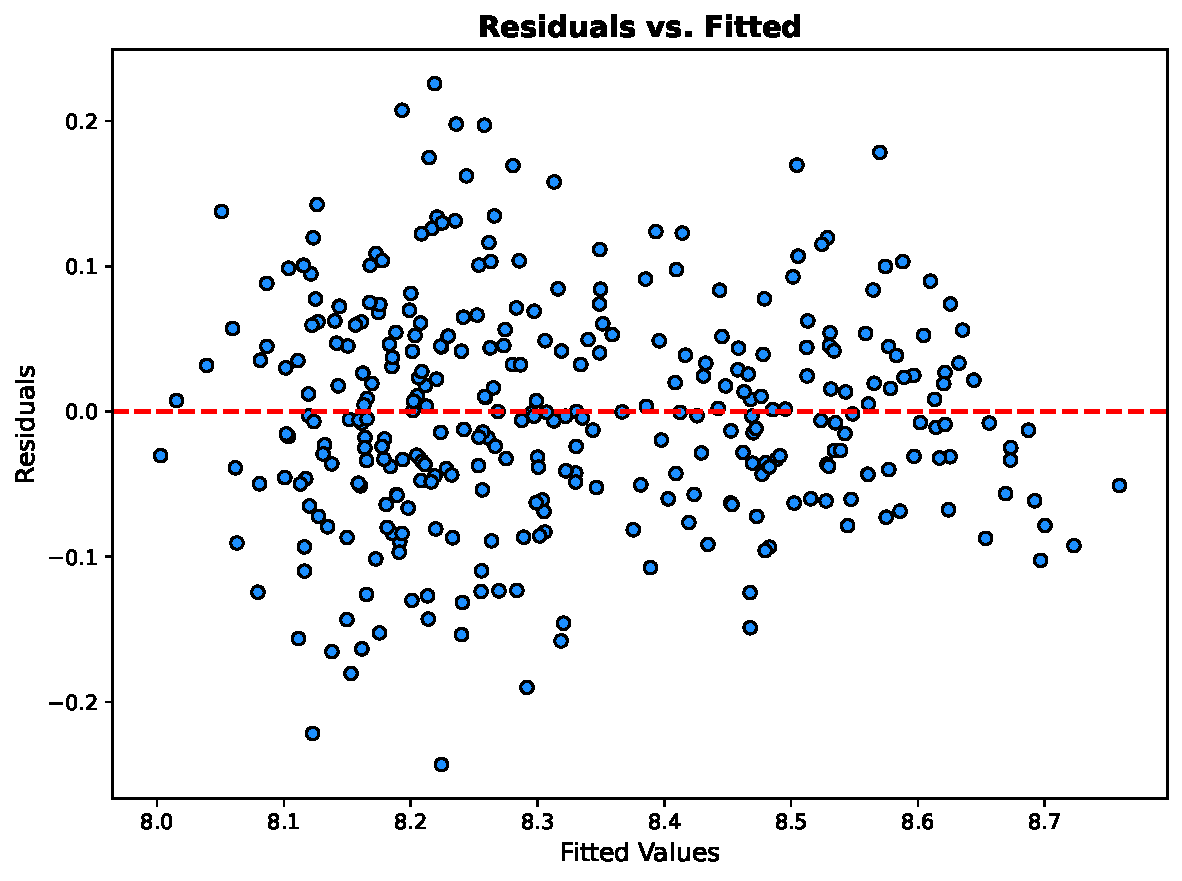
\includegraphics[width=0.6\textwidth,keepaspectratio]{./codes/plots/model-testing/res-vs-fit.pdf}
        \caption{Residuals vs. Fitted}
      \end{figure}

      \ii \textbf{Normal Q-Q Plot:} The standardized residuals
      tightly hug the theoretical $45$-degree diagonal line,
      visually indicating that the error terms are normally
      distributed.
      \begin{figure}[H]
        \centering
        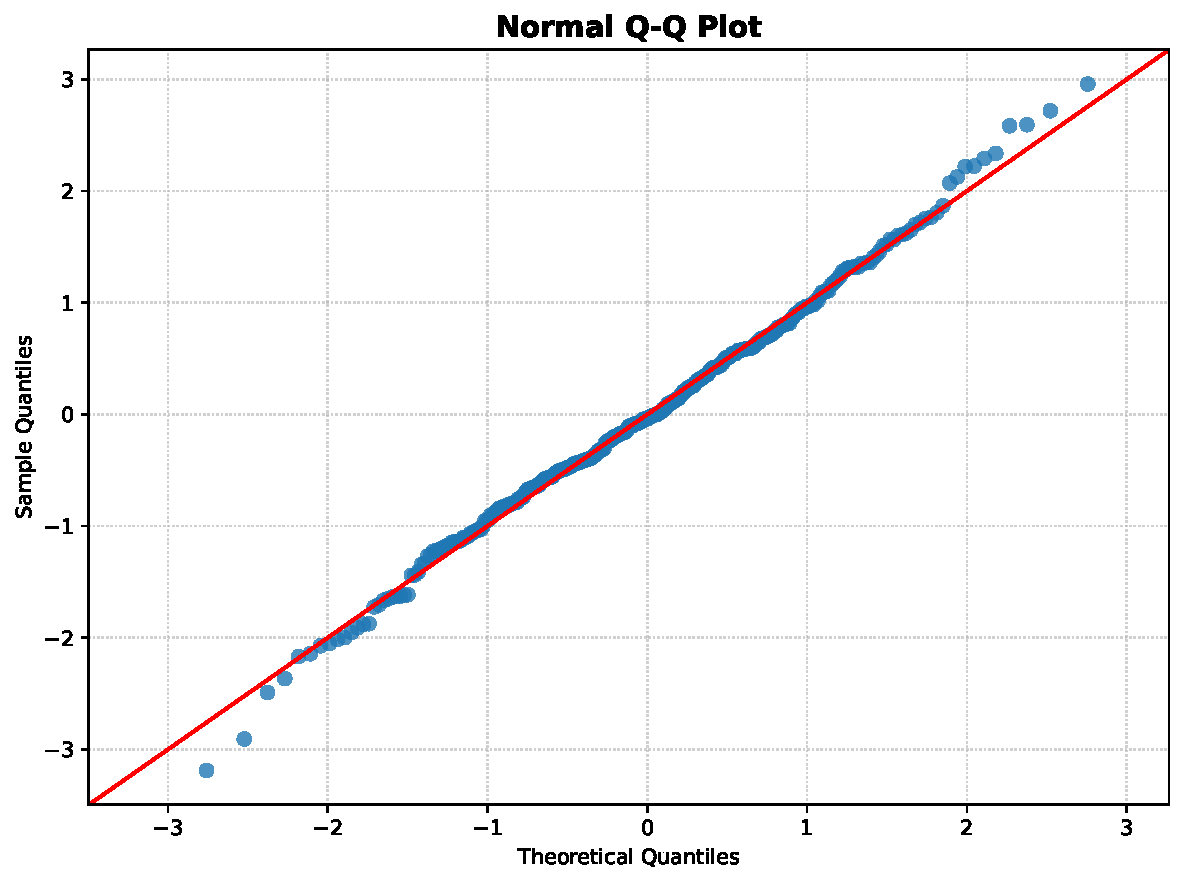
\includegraphics[width=0.6\textwidth,keepaspectratio]{./codes/plots/model-testing/qq-plot.pdf}
        \caption{Normal Q-Q Plot}
      \end{figure}
  \end{itemize}

  \subsubsection{Normality Assessment}
  To rigorously prove the visual assumption of normality
  established by the Q-Q plot, we apply the Pearson Chi-Square
  Goodness-of-Fit test to the model's standardized residuals.

  By standardizing the residuals ($\frac{\eps - \bar{\eps}}{s}$),
  we map them directly to a standard Normal distribution
  curve, $N(0,1)$. We slice this theoretical curve into $k=10$
  regions with equal probabilities, meaning the expected probability
  of a residual falling into any specific region is exactly
  $E_i = 10\%$.

  We then map our actual observed standardized residuals
  ($O_i$) into these regions. The test statistic evaluates the
  difference between the observed counts and the theoretically
  expected counts:
  \[
    \chi^2 = \sum_{i=1}^{k} \frac{(O_i - E_i)^2}{E_i}
    .\]

  \begin{figure}[H]
    \centering
    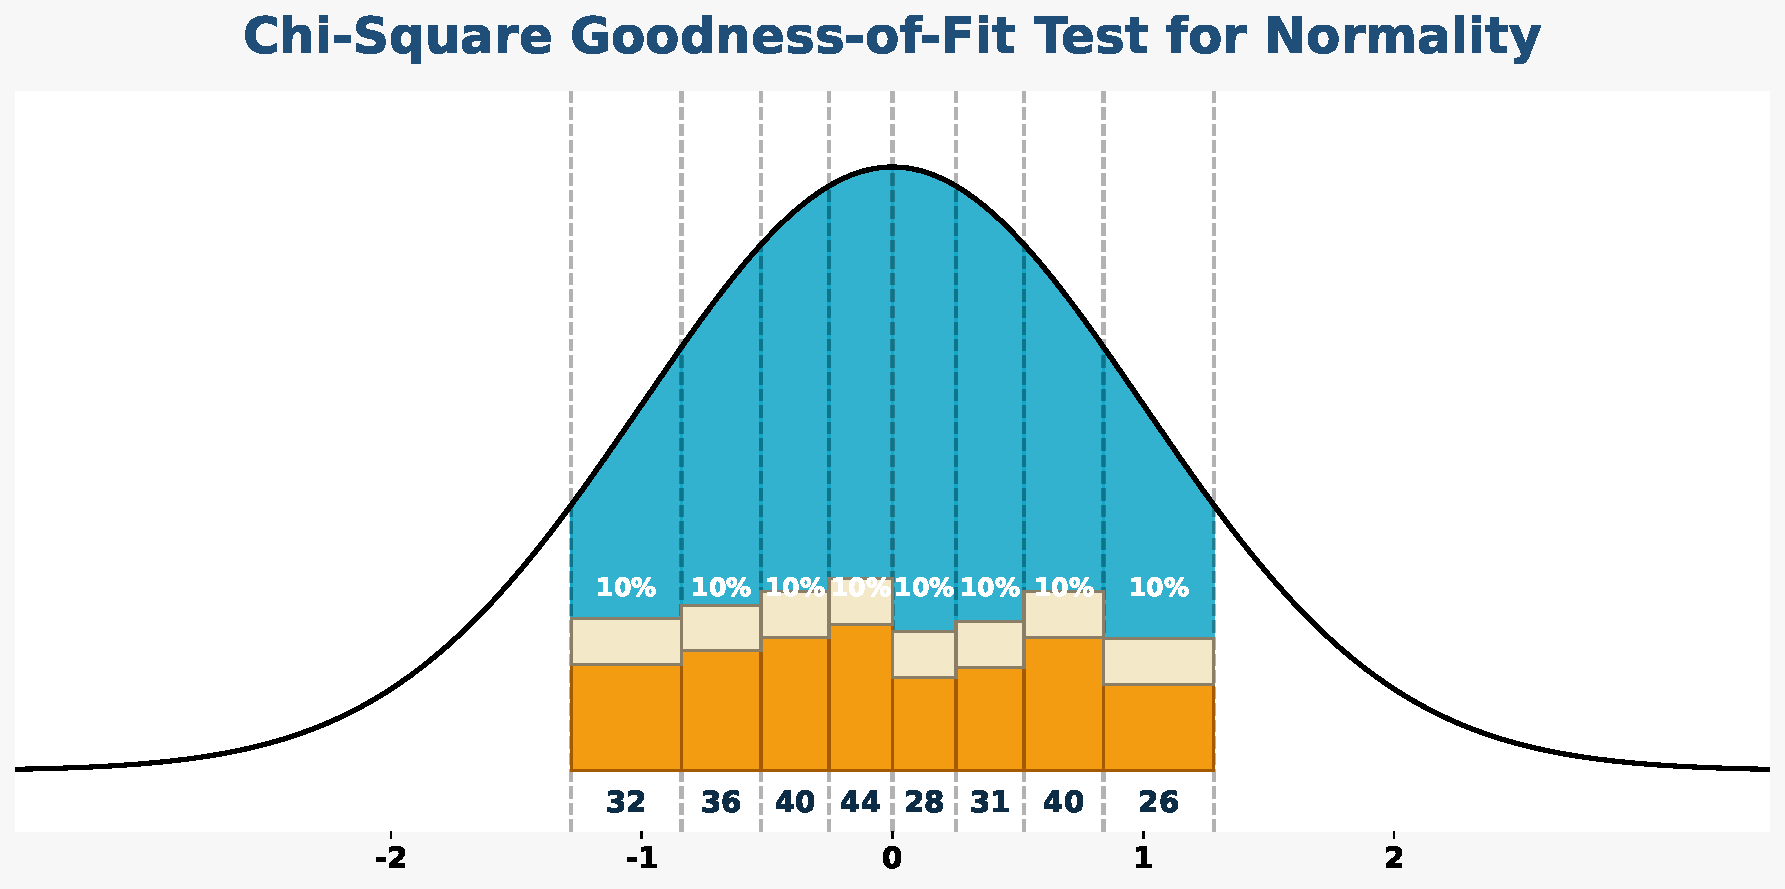
\includegraphics[width=0.8\textwidth,keepaspectratio]{./codes/plots/model-testing/pearson-chisq.pdf}
    \caption{Chi-Square Goodness-of-Fit Test for Normality}
  \end{figure}

  \paragraph{Calculation and Inference}
  Evaluating the standardized residuals across $10$ equiprobable
  bins yields a test statistic of $\chi^2 = 9.6374$. With
  $k-3 = 7$ degrees of freedom (accounting for the estimation
  of the mean and variance), this corresponds to a p-value of
  $0.2101$.

  Because this p-value is strictly greater than our significance
  threshold ($\alpha = 0.05$), we \textbf{fail to reject} the
  null hypothesis. This mathematically suggests that our residuals
  do not significantly deviate from a normal distribution.
  Consequently, all confidence intervals, prediction intervals,
  and hypothesis tests calculated in the preceding sections are
  reasonably supported.


  \section{Conclusion}

  This study developed a multiple linear regression model to
  explain penguin body mass using flipper length, culmen
  length, culmen depth, and species. Motivated by allometric
  scaling, a log transformation was applied to obtain a
  log-linear model that better captures the underlying
  relationships.

  The fitted model demonstrated strong explanatory power,
  accounting for about 83.5\% of the variation in log body
  mass. All predictors, except the intercept, were highly
  significant. Flipper length, culmen length, and culmen depth
  each showed a positive association with body mass, while the
  species indicators captured meaningful differences among
  penguin species.

  The inferential results supported the usefulness of the
  model. The overall F-test confirmed statistical significance,
  and the joint test showed that species provides additional
  explanatory power beyond physical measurements. Confidence
  and prediction intervals were consistent with the fitted
  model.

  Diagnostic analysis indicated that the regression assumptions
  are reasonably satisfied. Residual plots showed no major
  patterns, the Q-Q plot suggested approximate normality, and
  the chi-square test did not detect significant deviations.
  Overall, the model provides both strong predictive
  performance and a meaningful representation of the
  relationship between body mass and morphological traits.



  \appendix
  \section{Appendix}

  \subsection{Dataset}

  The dataset used in this study is the
  Palmer Penguins dataset\cite{palmerpenguins},
  originally collected by Kristen B.\ Gorman and made publicly
  available by Allison Marie Horst, Alison Presmanes Hill, and
  Kristen B.\ Gorman.

  It can be accessed through the following sources:
  \begin{itemize}
      \item GitHub:
      \href{https://github.com/allisonhorst/palmerpenguins}
      {github.com/allisonhorst/palmerpenguins}

      \item Kaggle:
      \href{https://www.kaggle.com/datasets/parulpandey/palmer-archipelago-antarctica-penguin-data}
      {kaggle.com/datasets/parulpandey/palmer-archipelago-antarctica-penguin-data}
  \end{itemize}

  \subsection{Code}

  The code used in this project is divided based on functionality:
  \begin{itemize}
      \item R Code (Computation and Model Fitting):
      \href{https://github.com/Bubu-Droid/mini-projects-repo/tree/main/lin-reg-sem-2/codes/r-codes}
      {R Code Link}

      \item Python Code (Visualization and Plotting):
      \href{https://github.com/Bubu-Droid/mini-projects-repo/tree/main/lin-reg-sem-2/codes/plots}
      {Python Code Link}
  \end{itemize}

  \bibliographystyle{plain}
  \bibliography{refs}

\end{document}
